% \subsection{Background}

%% cloud and virtualization technologies
Cloud computing was brought about by virtualization technologies,
enabling to build large pools of virtualized computing resources (e.g.,
servers, storage, and network) and dynamically allocate necessary resources
for providing services.
However, cloud computing system itself is still on physical cloud
infrastructure; cloud system operators manually manage
physical servers and network switches to meet the overall demands
so as not to overload certain resources.

The next challenge would be to virtualize cloud infrastructure!
By decoupling infrastructure management from service management,
cloud resources such as servers and networks can be provided with a
pay-as-you-go model.
Then, cloud service operators are liberated from hardware resource management,
as was the case for system administrators by cloud computing.
Moreover, it is not enough to shift responsibility to operators of the
new lower infrastructure layer. We need a new self-managing
infrastructure layer which does not require human operators.

%% Edge computing and micro datacenters
We also consider two recent trends in cloud computing.
One trend is edge computing~\cite{Lopez-2015} and
micro datacenters~\cite{Greenberg-2009}.
Small-scale datacenters with a few racks or even a couple of servers
can be placed at locations closer to the users, to reduce latencies
or to store sensitive data on premise, and make them act as part of
the cloud.
A possible future direction is distributed cloud computing that
utilizes diverse and geographically scattered computing resources.
It will require a new management mechanism to efficiently utilize such
resources.
On the other hand, computing resources will be abundant in the
environment so that it will be no longer necessary to micromanage
computing resources.

%% serverless, micro services
Another trend is microservices~\cite{nadareishvili2016microservice}
and serverless computing~\cite{Shafiei-2022} in which
a cloud service is composed of a collection of loosely-coupled
lightweight services.
Each microservice is ephemeral and short-lived, and can be executed
in a stateless container,
which enables flexible and efficient use of underlying cloud
resources.
The concept has something in common with early packet switching so
that it might open up new possibilities to apply packet switching
techniques to handling microservice jobs.

%% energy saving?
In addition, we should take energy saving into consideration as it is
essential for future clouds~\cite{Mastelic-2015,masanet2020recalibrating}.

\subsection{Cloud Morphing Vision}

\begin{figure}[tb]
  \begin{center}
    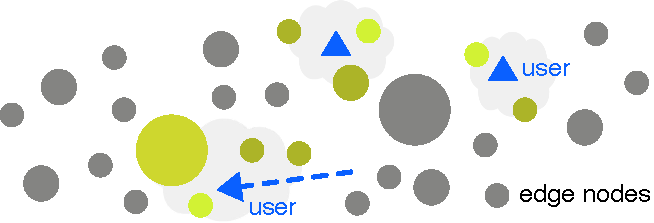
\includegraphics[width=0.8\columnwidth]{morphing-concept.pdf}
    \vspace{-2.0ex}
    \caption{Cloud morphing concept: the shape of a cloud follows the
      usage pattern}
    \Description{Clouds dynamically change their shapes.}
    \label{fig:concept}
  \end{center}
\end{figure}

{\em Cloud Morphing} is our vision for cloud virtualization in the future.
By dynamically allocating microservices over distributed
heterogeneous resources, a cloud service instance emerges at the best
location and, as the usage pattern changes, the service instance also
transforms the locations of the resources and their connections
(Figure \ref{fig:concept}).

Microservice jobs are assigned to reduce the execution cost that
consists of computing cost, communication cost with the user, access
cost to database, and other factors.
For examples, an interactive task will follow the user when the user
moves, while a data-intensive task will stay close to the data
regardless of the user location.
Edge computing is automatically formed by allocating resources close to
the users.
Moreover, services are inherently fault-tolerant and resilient
against outages or disasters since faulty resources are
automatically evicted from the resource pool.

From the operational perspective, the physical resource management
becomes simpler with a larger resource pool.
Physical nodes can be easily attached to or detached from the resource pool.
When there is a consistent hotspot, it can be alleviated or solved by
placing new resources close to the hotspot and then attaching them to
the resource pool at a convenient time.

Diverse resources would be owned and managed by different parties.
It requires loose management of resources, as small parties cannot
afford dedicated skilled operators.
The utilization of each resource needs to be easily manipulated,
without affecting the stability of the system.

To realize such systems, it requires various technical advances across
many fields.  Among other things, new autonomous resource management
model is needed for distributed diverse resources,
which is the topic of this paper.

\subsection{Resource Management}

%% resource allocation problems are NP-hard
%% even harder for distributed heterogeneous resources
Resource allocation in distributed clouds is a non-trivial
optimization problem, and it is even harder when distributed
management is assumed.
%% our idea: use congestion pricing mechanism for automatic load management
To this end, we employ dynamic pricing for decentralized resource
allocation which works as backpressure against congestion.
By design, serious congestion never happens in the system as long as
some resources remain available in the resource pool.
It also reserves a sufficient margin essential for the performance of
statistically multiplexing services.
We use pseudo cost for manipulating resource allocation.
Here, pseudo cost is not an actual monetary charge, but it is used to
control resource utilization.
There exists a large body of literature formulating resource allocation
as optimization problems.
In this paper, we use terms and expressions borrowed from optimization
theory. Our goal is, however, not to pursue theoretical optimum
allocations, but to present a practical feedback control model for
distributed resource management.


